\documentclass{article}
\usepackage[usenames]{color} %used for font color
\usepackage{amsfonts}
\usepackage{amsmath}
\usepackage{amssymb}
\usepackage{array}
% \usepackage{amsthm}
\usepackage{bm}
\usepackage{bbm}
\usepackage{booktabs}
\usepackage{cite}
\usepackage{CJKutf8}
\usepackage{color}
\usepackage{comment}
\usepackage{courier}
\usepackage{enumerate}
\usepackage{enumitem}
\usepackage{epsfig}
\usepackage{eurosym}
\usepackage{float}
\usepackage[stable]{footmisc}
% \usepackage[bottom]{footmisc}
\usepackage[top=2.5cm,bottom=2.5cm,left=2.5cm,right=2.5cm]{geometry}
\usepackage{graphicx}  
\usepackage{helvet}
\usepackage{hhline}
\usepackage{hyperref}
\usepackage{imakeidx} % allows index generation
\usepackage{latexsym}
\usepackage{mathdots}
\usepackage{mathptmx}
\usepackage{microtype}
\usepackage{multicol}
\usepackage{multirow}
\usepackage{palatino}
\usepackage{pgfplots}
\pgfplotsset{compat=newest}
\usepackage{pdfsync}
\usepackage{psfrag}
\usepackage{pstricks}
\usepackage{subfigure}
\usepackage[many]{tcolorbox}
\usepackage{tikz,pgf}
\usetikzlibrary{backgrounds}
\usetikzlibrary{plotmarks}
\usepackage{tikz-layers}
\usepackage{type1cm}
\usepackage{ulem}
\usepackage{yfonts}


\def\x{\mathbf{x}}


\def\y{\mathbf{y}}
\def\c{\mathbf{c}}
\def\d{\mathbf{d}}
\def\A{\mathbf{A}}
\def\B{\mathbf{B}}
\def\b{\mathbf{b}}
\def\y{\mathbf{y}}
\def\Re{\mathbb{R}}
\def\Z{\mathbb{Z}}


\title{ISyE 6669 HW 15}
\date{Fall 2025}
\begin{document}
\maketitle

\begin{enumerate}
    \item Let \( x_1, x_2, x_3 \) be continuous nonnegative variables with values in the range \([0, 10]\). Write a set of constraints to model the requirement
that:
\[
|2x_1 - x_2 - x_3| \geq 2
\]
by introducing an additional binary variable. 
 \item Let $x_1, x_2, x_3$ be binary variables with the following relationship:
 \begin{table}[h!]
\centering
\begin{tabular}{|c|c|c|}
\hline
\( x_1 \) & \( x_2 \) & \( x_3  \) \\
\hline
0 & 0 & 0 \\
0 & 1 & 1 \\
1 & 0 & 1 \\
1 & 1 & 0 \\
\hline
\end{tabular}
\caption{Truth table for XOR operation}
\end{table}
\begin{enumerate}
\item In the following formulation correct? Explain what each constraint is doing?
\begin{eqnarray*}
(1 - x_1) + x_2 + x_3 &\geq & \frac{1}{2}\\
x_1 + (1 - x_2) + x_3 &\geq & \frac{1}{2}\\
x_1 + x_2 + (1 - x_3) & \geq & \frac{1}{2}\\
(1 - x_1) + (1 - x_2) + (1 - x_3) &\geq& \frac{1}{2}\\
\end{eqnarray*}
\item Can you write a formulation using \emph{one equation}? Hint: You may need to use an additional  variable. 
 \end{enumerate}
 \item A plantation is in the business of commercially growing and harvesting trees for lumber. The plantation is divided into 10 grids as shown below:
\begin{center}
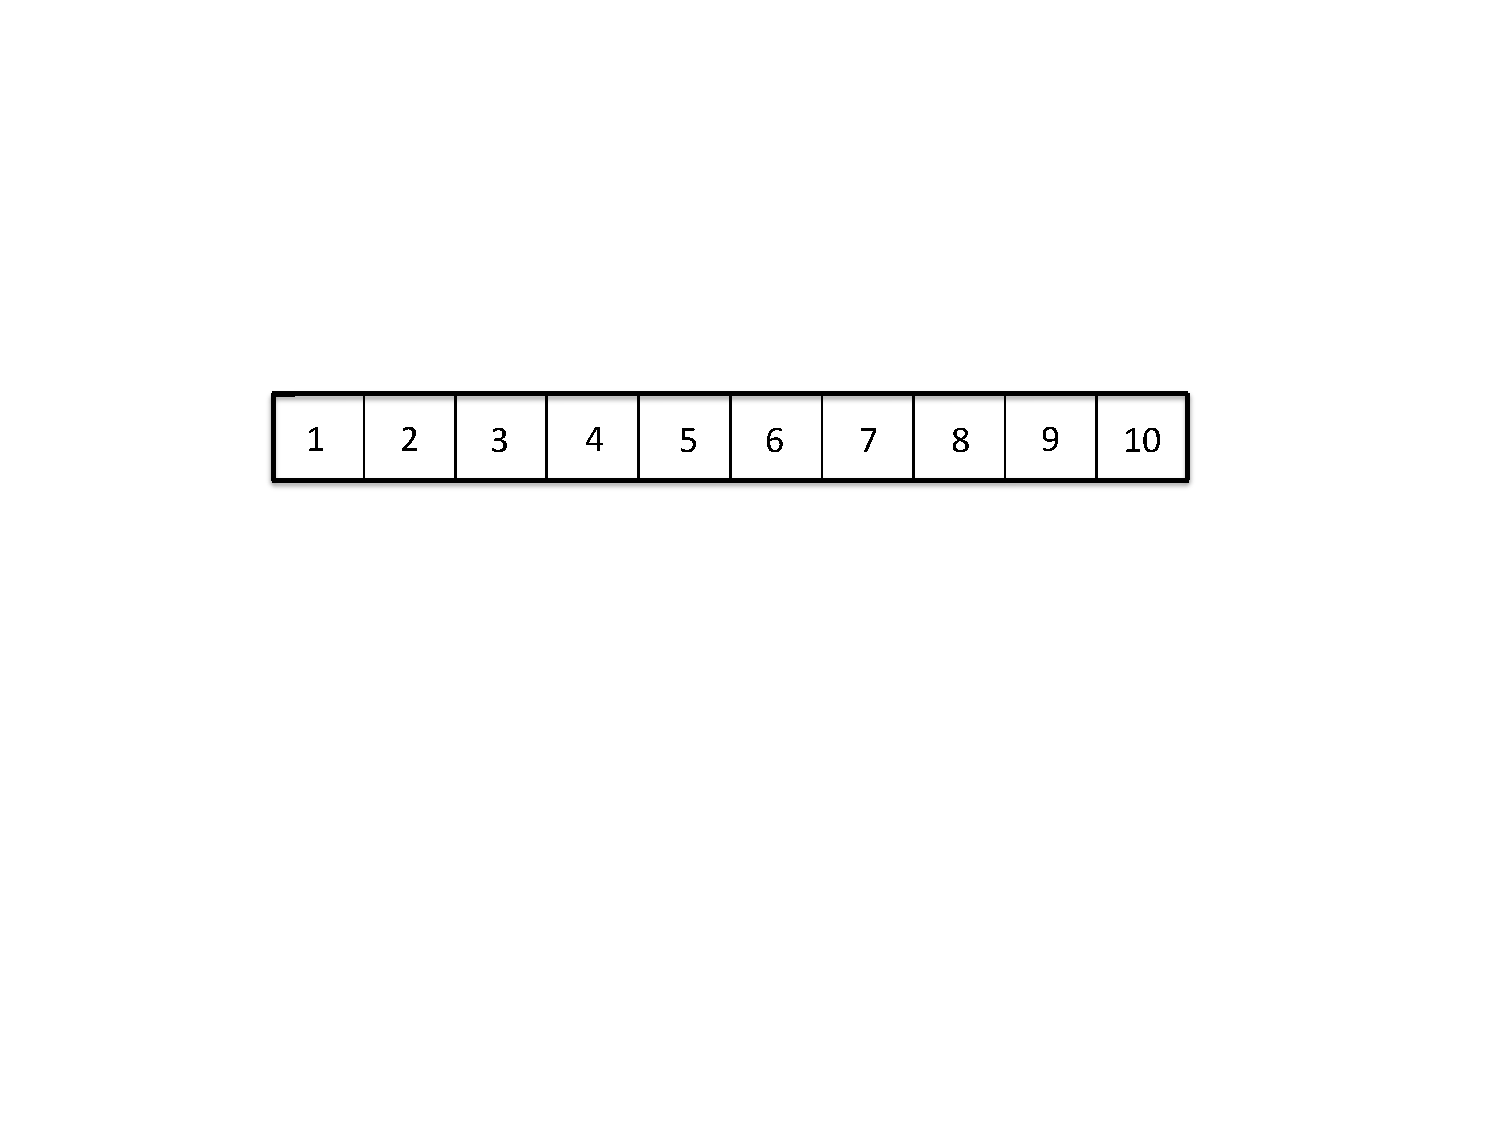
\includegraphics[width = 0.7\textwidth]{figures1.pdf}
\end{center}
We are planning for the next four years. Each year, the plantation cuts all the trees in some of the grids and then replants trees in these grids in the same year. Use the following decision variable:
$$x_{it} = \left\{\begin{array}{cl} 1& \textup{if trees in grid }i\textup{ are harvested in year }t\\ 0 & \textup{otherwise}\end{array}\right.$$
\begin{enumerate}
\item A profit of $p_{it}$ is earned if the grid $i$ is harvested in time period $t$. Write down a linear objective function that represents maximizing total profit.
\item No more than 6 grids can be harvested in a single year.  Write  linear inequalities to model this constraint.
\item  Because trees need time to grow, each grid may be harvested at most 2 times over the next four years, and it may not be harvested in consecutive years. Write linear inequalities to model these constraints.
\item  Ecological considerations require the implementation of following rule: In any given year, the set of unharvested grids must be connected. For example: harvesting grids $1, 2, 5, 6$ in time period 1 is not allowed since the unharvested grids are disconnected into two blocks $3, 4$ and $7,8,9,10$. Write linear inequalities to represent the above constraints. You may introduce artificial variables as necessary. 
\end{enumerate}


 \item A hospital is scheduling nurses for aiding in surgery. 10 surgeries need to be performed. Each surgery requires exactly 2 nurses. There are 25 available nurses. We have the following additional constraints.
\begin{enumerate}
\item A nurse can aid in a surgery only if the nurse is qualified to do so. The following data is available: $d_{ij} = 1$ if nurse $i$ is qualified to aid in surgery $j$ and $d_{ij} = 0$ if nurse $i$ is not qualified to aid in surgery $j$ ($d_{ij}$ provided for all $i = 1, ....25$ and for all $j = 1, ..., 10$).
\item Nurse 1, Nurse 2, ..., Nurse 15 are senior nurses. Nurses 16, ..., Nurse 25 are junior nurses. Each surgery must have at least 1 senior qualified nurse.
\item  Nurse 1 and Nurse 20 do not work well together. They must not be scheduled to the same surgery.
\item Each nurse can aid in at most 2 surgeries.
\item At least 5 junior nurses must be aiding surgeries.
\end{enumerate}
Formulate an integer program to find a feasible schedule.

\item Consider the following branch-and-bound tree for solving a two variable integer programming problem.

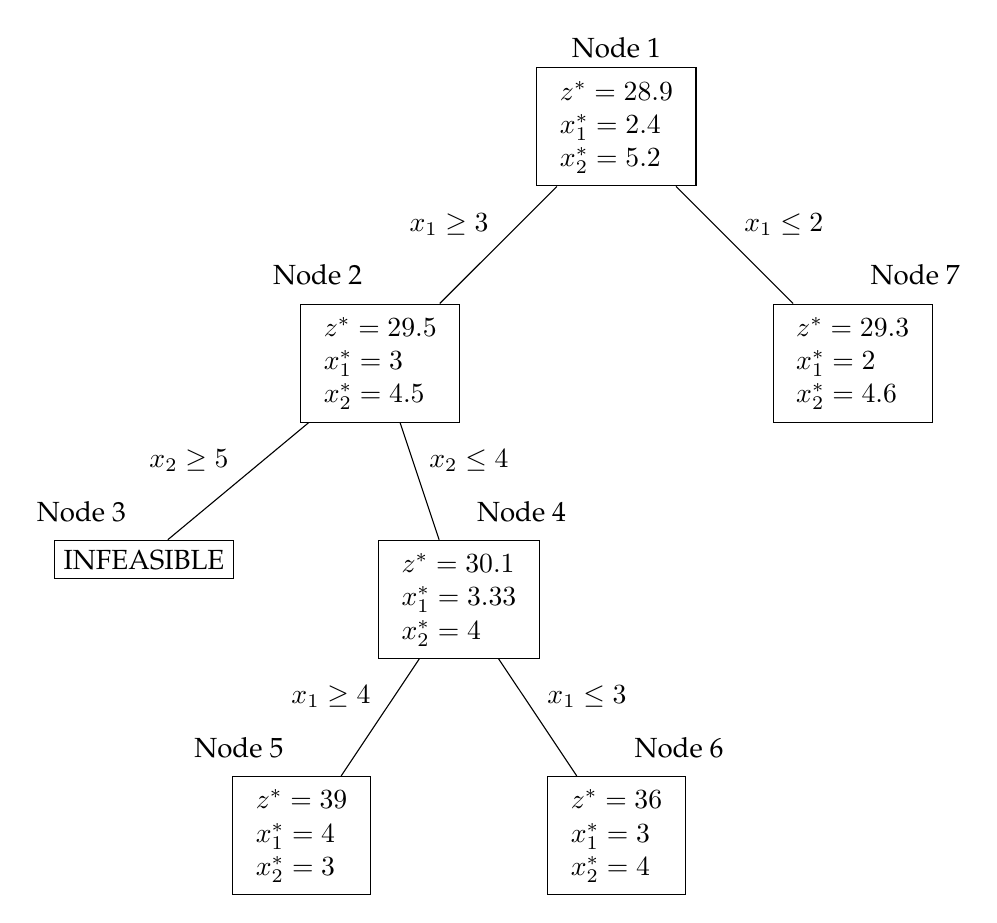
\begin{tikzpicture}[scale=1]

\draw (0,0) node[shape=rectangle,draw,anchor=north] (n1)
{$\begin{array}{l} z^* = 28.9 \\ x_1^*=2.4 \\ x_2^* = 5.2
\end{array}$}-- node[above] {Node 1} (n1);


\draw (-3,-3) node[shape=rectangle,draw,anchor=north] (n2)
{$\begin{array}{l} z^* = 29.5 \\ x_1^*=3 \\ x_2^* = 4.5
\end{array}$} -- node[above left=3pt] {Node 2} (n2) ;


\draw (-6,-6) node[shape=rectangle,draw,anchor=north] (n3)
{\vspace{0.2in}\\

INFEASIBLE \\

\vspace{0.2in} } -- node[above left=3pt] {Node 3} (n3) ;


\draw (-2,-6) node[shape=rectangle,draw,anchor=north] (n4)
{$\begin{array}{l} z^* = 30.1 \\ x_1^*=3.33 \\ x_2^* = 4
\end{array}$} -- node[above right=3pt] {Node 4} (n4) ;


\draw (-4,-9) node[shape=rectangle,draw,anchor=north] (n5)
{$\begin{array}{l} z^* =39 \\ x_1^*=4 \\ x_2^* = 3
\end{array}$} -- node[above left=3pt] {Node 5} (n5) ;

\draw (0,-9) node[shape=rectangle,draw,anchor=north] (n6)
{$\begin{array}{l} z^* = 36 \\ x_1^*=3 \\ x_2^* = 4
\end{array}$} -- node[above right=3pt] {Node 6} (n6) ;

\draw (3,-3) node[shape=rectangle,draw,anchor=north] (n7)
{$\begin{array}{l} z^* = 29.3 \\ x_1^*=2 \\ x_2^* = 4.6
\end{array}$} --
node[above right=3pt] {Node 7} (n7);

\draw (n1) -- node[anchor=south east]{$x_1 \geq 3$} (n2);

\draw (n1) -- node[anchor=south west]{$x_1 \leq 2$} (n7);

\draw (n2) -- node[anchor=south east]{$x_2 \geq 5$} (n3);

\draw (n2) -- node[anchor=south west]{$x_2 \leq 4$} (n4);

\draw (n4) -- node[anchor=south east]{$x_1 \geq 4$} (n5);

\draw (n4) -- node[anchor=south west]{$x_1 \leq 3$} (n6);

\end{tikzpicture}

\begin{enumerate}
\item  Is this a minimization or a maximization problem?
\item  For each of the following nodes, indicate whether you need to further branch on the node.
\begin{itemize}
    \item[] Node 3:
    \item[] Node 5:
    \item[] Node 7:
\end{itemize}
\item According to this branch-and-bound tree, what is the range (lower and upper bounds) in which the optimal IP value lies? Explain your answer.
\end{enumerate}
 
\end{enumerate}

\end{document}

